\documentclass[12pt]{exam}
\usepackage[margin=1in]{geometry}
\usepackage{amsmath}
\usepackage{amsfonts}
\usepackage{tikz}
\usepackage{multicol}
\usepackage{tasks}
\usepackage{xcolor}

% Custom solution formatting
\shadedsolutions
\definecolor{SolutionColor}{gray}{0.9}

\begin{document}

% Replaced custom \quizfrontpage with standard LaTeX equivalent
\begin{center}
\fbox{\fbox{\parbox{5.5in}{\centering Pre-Calculus 11 - Inequalities Check-in Quiz}}}
\\
\vspace{5mm}
\makebox[0.75\textwidth]{Name :\enspace\hrulefill}

\vspace{3mm}
\makebox[0.75\textwidth]{Teacher's name:\enspace\hrulefill}
\end{center}

\begin{questions}

\question Write the inequality represented by each number line using \textbf{interval notation}.
\begin{tasks}(2)
    \task \\
    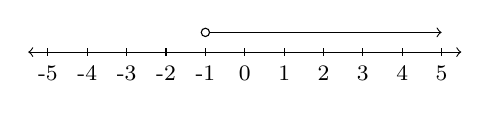
\begin{tikzpicture}[scale=0.5]
        \draw[<->] (-5.5,0) -- (5.5,0);
        \foreach \x in {-5,-4,-3,-2,-1,0,1,2,3,4,5} \draw (\x,0.1) -- (\x,-0.1) node[below] {\footnotesize \x};
        \draw (-1,0.5) circle(3pt); \draw[->] (-0.9,0.5)--(5,0.5);
    \end{tikzpicture}
    \task \\
    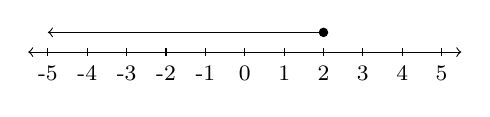
\begin{tikzpicture}[scale=0.5]
        \draw[<->] (-5.5,0) -- (5.5,0);
        \foreach \x in {-5,-4,-3,-2,-1,0,1,2,3,4,5} \draw (\x,0.1) -- (\x,-0.1) node[below] {\footnotesize \x};
        \filldraw (2,0.5) circle(3pt); \draw[->] (1.9,0.5)--(-5,0.5);
    \end{tikzpicture}
    \end{tasks}
    \vspace{\stretch{1}} % Replaced \svert[1]
    \begin{tasks}[resume](2)
    \task \\
    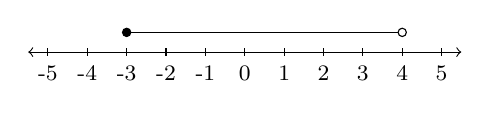
\begin{tikzpicture}[scale=0.5]
        \draw[<->] (-5.5,0) -- (5.5,0);
        \foreach \x in {-5,-4,-3,-2,-1,0,1,2,3,4,5} \draw (\x,0.1) -- (\x,-0.1) node[below] {\footnotesize \x};
        \filldraw (-3,0.5) circle(3pt); \draw (4,0.5) circle(3pt); \draw[] (-2.9,0.5)--(3.9,0.5);
    \end{tikzpicture}
    \task \\
    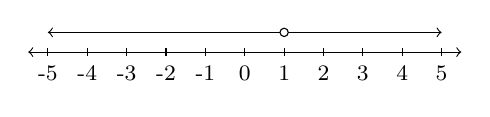
\begin{tikzpicture}[scale=0.5]
        \draw[<->] (-5.5,0) -- (5.5,0);
        \foreach \x in {-5,-4,-3,-2,-1,0,1,2,3,4,5} \draw (\x,0.1) -- (\x,-0.1) node[below] {\footnotesize \x};
        \draw (1,0.5) circle(3pt); \draw[->] (0.9,0.5)--(-5,0.5); \draw[->] (1.1,0.5)--(5,0.5);
    \end{tikzpicture}
    \vspace{\stretch{1}} % Replaced \svert[1] at the end of the tasks block
\end{tasks}
\begin{solution}
\begin{tasks}(2)
    \task $(-1, \infty)$
    \task $(-\infty, 2]$
    \task $[-3, 4)$
    \task $(-\infty, 1) \cup (1, \infty)$ or $x \neq 1$
\end{tasks}
\end{solution}
\vspace{\stretch{1}} % Replaced \svert[1]

\question Represent the following values on a number line.
\begin{tasks}(2)
    \task $x \in [-5, 0)$ \\
    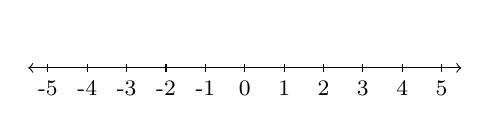
\begin{tikzpicture}[scale=0.5,baseline={([yshift=3ex]current bounding box.north)}]
        \draw[<->] (-5.5,0) -- (5.5,0);
        \foreach \x in {-5,-4,-3,-2,-1,0,1,2,3,4,5} \draw (\x,0.1) -- (\x,-0.1) node[below] {\footnotesize \x};
    \end{tikzpicture}
    \task $\{x\mid x\leq 4\}$ \\ 
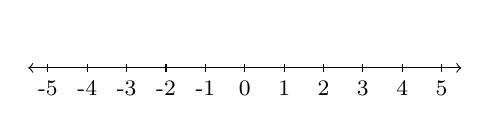
\begin{tikzpicture}[scale=0.5,baseline={([yshift=3ex]current bounding box.north)}]        
    \draw[<->] (-5.5,0) -- (5.5,0);
        \foreach \x in {-5,-4,-3,-2,-1,0,1,2,3,4,5} \draw (\x,0.1) -- (\x,-0.1) node[below] {\footnotesize \x};
    \end{tikzpicture}
    \end{tasks}
    \begin{tasks}[resume](2)
    \task $x \in (-\infty, 2] \cup [4, \infty)$
    \\
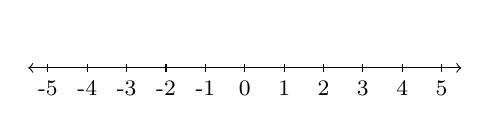
\begin{tikzpicture}[scale=0.5,baseline={([yshift=3ex]current bounding box.north)}]        
    \draw[<->] (-5.5,0) -- (5.5,0);
        \foreach \x in {-5,-4,-3,-2,-1,0,1,2,3,4,5} \draw (\x,0.1) -- (\x,-0.1) node[below] {\footnotesize \x};
    \end{tikzpicture}
    \task $\{x\in\mathbb{Z}\mid -2<x\leq 3\}$
    \\
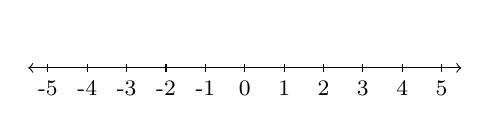
\begin{tikzpicture}[scale=0.5,baseline={([yshift=3ex]current bounding box.north)}]        
    \draw[<->] (-5.5,0) -- (5.5,0);
        \foreach \x in {-5,-4,-3,-2,-1,0,1,2,3,4,5} \draw (\x,0.1) -- (\x,-0.1) node[below] {\footnotesize \x};
    \end{tikzpicture}
\end{tasks}
\begin{solution}
\begin{tasks}(2)
\end{tasks}
\end{solution}

\question Solve the following linear inequalities. Express your final answer in \textbf{interval notation}.
\begin{tasks}(2)
    \task $-3x + 12 < 24$
    \task $5(x - 2) \geq 7x + 4$
\end{tasks}
\begin{solution}
\begin{tasks}(2)
    \task $-3x < 12 \implies x > -4 \implies (-4, \infty)$
    \task $5x - 10 \geq 7x + 4 \implies -2x \geq 14 \implies x \leq -7 \implies (-\infty, -7]$
\end{tasks}
\end{solution}
\vspace{\stretch{1}} % Replaced \svert[1]

\pagebreak

\question Solve the following quadratic inequalities algebraically (using a sign chart or sketching). Express your answers in \textbf{interval notation}.
\begin{tasks}(2)
    \task $x^2 + 2x - 8 \leq 0$
    \task $x^2 - 9 > 0$
    \end{tasks}
    \vspace{\stretch{1}} % Replaced \svert[1]
    \begin{tasks}[resume](2)
    \task $2x^2 - 5x - 3 \geq 0$
    \task $-x^2 + 6x - 5 < 0$
\end{tasks}
\begin{solution}
\begin{tasks}(2)
    \task $(x+4)(x-2) \leq 0 \implies [-4, 2]$
    \task $(x-3)(x+3) > 0 \implies (-\infty, -3) \cup (3, \infty)$
    \task $(2x+1)(x-3) \geq 0 \implies (-\infty, -1/2] \cup [3, \infty)$
    \task $x^2 - 6x + 5 > 0 \implies (x-5)(x-1) > 0 \implies (-\infty, 1) \cup (5, \infty)$
\end{tasks}
\end{solution}
\vspace{\stretch{1}} % Replaced \svert[1]

\question Solve the following inequalities.
\begin{tasks}(2)
    \task $x^2 + 6x + 9 > 0$
    \task $x^2 + 5 \leq 0$
\end{tasks}
\begin{solution}
\begin{tasks}(2)
    \task $(x+3)^2 > 0$. True for all $x$ except $-3$: $(-\infty, -3) \cup (-3, \infty)$
    \task A parabola shifted up 5 will never be $\leq 0$. \textbf{No Solution} ($\emptyset$)
\end{tasks}
\end{solution}
\vspace{\stretch{1}} % Replaced \svert[1]
\end{questions}
\end{document}